\chapter{Interacting Fields}

Free theories are a good starting point to understand the basic concepts and techniques of quantum field theory, but to capture the full complexity of the physical world, we need to introduce interactions between fields. Interactions allow us to describe processes such as scattering, particle decays, and the formation of bound states, which are essential for understanding the behavior of matter and energy at a fundamental level.
In a free theory, the fields do not interact with each other, and the equations of motion are linear: they can exhibit \textit{at most quadratic terms in the fields} (in the lagrangian \(\mathcal{L}\)). We can then build interacting theories by adding non-linear terms to the Lagrangian, which will lead to non-linear equations of motion. These non-linearities are what give rise to the rich phenomenology of interacting quantum field theories.

The most important tools in the developing of interacting quantum field theories are:
\begin{itemize}
    \item \textbf{Dimensional analysis}, which allows us to determine the relevance of different interaction terms at different energy scales, and to classify interactions as relevant, irrelevant, or marginal.
    \item \textbf{Renormalization}, which is a systematic procedure to deal with the infinities that arise in perturbative calculations of interacting theories, and to extract meaningful physical predictions from them.
    \item \textbf{Symmetry principles}, which play a crucial role in constraining the form of the interactions and in determining the properties of the particles and fields in the theory. For example, gauge symmetries lead to the introduction of gauge fields, which mediate the fundamental forces of nature.
\end{itemize}

Moreover \textbf{locality} is a fundamental principle in quantum field theory, which states that interactions should occur at the same point in spacetime. This principle ensures that the theory respects causality and allows us to construct a consistent framework for describing the dynamics of fields and particles:
\[
    \mathcal{L}(x) = \mathcal{L} \left( \phi(x), \partial_\mu \phi(x) \right), \quad \mathcal{L}(x) \neq \mathcal{L} \left( \phi(x+y), \partial_\mu \phi(x+y) \right),
\]
and the interaction terms we will introduce will be local, meaning that they will involve products of fields and their derivatives evaluated at the same spacetime point \(x\); this ensures that the theory is consistent with the principles of special relativity and quantum mechanics, and it will guide us in constructing the interaction terms in the Lagrangian.

In the next section we will start by performing a dimensional analysis of the fields and the interaction terms, which will help us to understand the behavior of the theory at different energy scales and to identify the most relevant interactions for describing physical phenomena. This will set the stage for our subsequent discussions on renormalization and symmetry principles in interacting quantum field theories.

\section{Dimensional Analysis}

In physics, and particularly in High Energy Physics (HEP), we heavily rely on the system of Natural Units where we set the reduced Planck constant and the speed of light to unity: \(\hbar = c = 1\). Consequently, mass, energy, momentum, inverse length, and inverse time all share the exact same dimension. There is only one independent dimensional unit left, which we conventionally identify with the dimension of mass.

We define the \textbf{mass dimension} of a generic quantity \(X\) as \([X]\). By definition:
\[
    [\text{mass}] = 1
\]
From the uncertainty principle or the De Broglie relations (\(x \sim \hbar/p\), \(t \sim \hbar/E\)), coordinates in space and time have an inverse mass dimension:
\[
    [x] = [t] = [\text{length}] = [\text{mass}^{-1}] = -1
\]
Because \(\hbar = 1\) is completely dimensionless, the physical action \(S\) must also be strictly dimensionless:
\[
    [S] = 0
\]
Since the action is the integral of the Lagrangian density over 4-dimensional spacetime (\(S = \int d^4x \, \mathcal{L}\)), and the integration measure \([d^4x] = [x^0 x^1 x^2 x^3] = -4\), we immediately deduce the fundamental mass dimension of the Lagrangian density:
\[
    [\mathcal{L}] = +4
\]
From this requirement, combined with the fact that \([m] = [\partial_\mu] = 1\), we can systematically derive the mass dimension of any quantum field simply by inspecting its free kinetic Lagrangian.
\begin{itemize}
    \item \textbf{Scalar (Spin-0) and Vector (Spin-1) fields:}
          The kinetic terms are proportional to \((\partial \phi)^2\) and \((\partial A)^2\). Therefore, \(2 + 2[\phi] = 4 \implies [\phi] = [A^\mu] = 1\).
    \item \textbf{Dirac Spinors (Spin-1/2):}
          The kinetic term involves only one derivative, \(\bar{\psi}\slashed{\partial}\psi\). Therefore, \(1 + 2[\psi] = 4 \implies [\psi] = 3/2\).
\end{itemize}

\subsection{Examples of Interaction Terms}

The total Lagrangian for an interacting quantum field theory takes the general form:
\[
    \mathcal{L} = \mathcal{L}_{\text{FREE}} + \mathcal{L}_{\text{INT}}
\]
where \(\mathcal{L}_{\text{FREE}}\) is the sum of all free, quadratic Lagrangians for the fields involved in the theory. The interaction part, \(\mathcal{L}_{\text{INT}}\), can be written as a sum over various interaction operators:
\[
    \mathcal{L}_{\text{INT}} = \sum_j g_j \mathcal{O}_j(\phi_k, \partial_\mu \phi_k)
\]
Here, \(\mathcal{O}_j\) is a composite \textbf{operator} (a product of fields and possibly their derivatives). Crucially, these operators must be \textit{Lorentz scalars} to preserve the Lorentz invariance of the action. The coefficients \(g_j\) are the \textbf{coupling constants}, which dictate the strength of the interaction.

Because the total Lagrangian must have dimension 4, we have a strict constraint on the dimensions of the couplings and the operators:
\[
    4 = [\mathcal{L}] = [g_j] + [\mathcal{O}_j] \implies [g_j] = 4 - [\mathcal{O}_j]
\]
This relation implies that the higher the mass dimension of the interaction operator \(\mathcal{O}_j\), the lower (more negative) the mass dimension of its associated coupling constant \(g_j\).

\begin{remark}
    Theories containing at least one coupling constant with a negative mass dimension (\([g_j] < 0\), which is completely equivalent to having an operator with \([\mathcal{O}_j] > 4\)) are classified as \textbf{non-renormalizable}. These theories become un-predictive at very high energy scales because they require an infinite number of counterterms to absorb ultraviolet divergences. However, they can still be incredibly useful as \textit{Effective Field Theories} (EFTs), yielding highly accurate physical predictions at lower energies.
\end{remark}

\subsubsection*{The Symmetries Dictate the Interactions}
A fundamental question arises: which specific operators \(\mathcal{O}_j\) should be included in \(\mathcal{L}_{\text{INT}}\)? The golden rule of modern QFT is:
\begin{center}
    \textit{One must include ALL operators that respect the underlying symmetries of the theory, up to a chosen maximal mass dimension \([\mathcal{O}_j] \leq d_{\text{max}}\).}
\end{center}
Usually, for a fundamental renormalizable theory, we set \(d_{\text{max}} = 4\). For effective theories, \(d_{\text{max}}\) is an integer strictly greater than 4. The profound reason behind this requirement is that quantum corrections (loop diagrams) will inevitably generate every possible interaction term allowed by the symmetries, even if we manually set them to zero at the classical tree-level. This is why we state that \textit{symmetries uniquely define the theory}.

\subsubsection{\(\phi^3\) Theory}

For pedagogical purposes, we often consider a simplified model known as \(\phi^3\) theory, which describes a single real scalar field self-interacting via a cubic potential.
\[
    \mathcal{L} = \mathcal{L}_{\text{K.G.}} + \mathcal{L}_{\text{INT}} = \frac{1}{2}(\partial_\mu \phi)^2 - \frac{1}{2}m^2\phi^2 - \frac{\lambda}{3!}\phi^3
\]
In this specific theory:
\begin{itemize}
    \item \(\phi^3\) is the cubic interaction operator. Its mass dimension is \([\phi^3] = 3 \times 1 = 3\).
    \item \(\lambda\) is the coupling constant. Its mass dimension is \([\lambda] = 4 - 3 = 1\).
    \item The factor \(1/3!\) is a conventional symmetry prefactor that elegantly cancels combinatorial factors when calculating Feynman diagrams.
\end{itemize}

Despite its mathematical simplicity, \textbf{this theory is fundamentally unphysical}. To see why, we compute the classical Hamiltonian density (the energy density). The conjugate momentum is \(\pi \equiv \frac{\partial \mathcal{L}}{\partial \dot{\phi}} = \dot{\phi}\).
\[
    \mathcal{H} = \pi \dot{\phi} - \mathcal{L} = \frac{1}{2}\pi^2 + \frac{1}{2}(\nabla \phi)^2 + \frac{1}{2}m^2\phi^2 + \frac{\lambda}{3!}\phi^3
\]
The potential energy density is \(V(\phi) = \frac{1}{2}m^2\phi^2 + \frac{\lambda}{3!}\phi^3\).

\begin{figure}[H]
    \centering
    \begin{minipage}{0.48\textwidth}
        \centering
        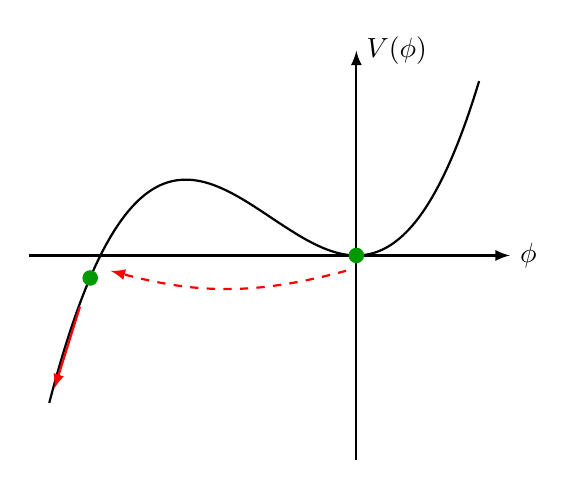
\begin{tikzpicture}[scale=1.3, > = latex]
            \draw[->, thick] (-3.2, 0) -- (1.5, 0) node[right] {$\phi$};
            \draw[->, thick] (0, -2) -- (0, 2) node[right] {$V(\phi)$};

            \draw[thick, domain=-3.0:1.2, smooth, samples=100] plot ({\x}, {0.8*\x*\x + 0.32*\x*\x*\x});

            \filldraw[green!60!black] (0,0) circle (2pt);

            \filldraw[green!60!black] (-2.6, -0.22) circle (2pt);

            \draw[->, dashed, thick, red] (-0.1, -0.15) to[bend left=15] (-2.4, -0.15);

            \draw[->, thick, red] (-2.7, -0.5) -- (-2.95, -1.3);
        \end{tikzpicture}
    \end{minipage}\hfill
    \begin{minipage}{0.48\textwidth}
        \caption{Plot of the scalar potential $V(\phi) = \frac{1}{2}m^2\phi^2 + \frac{\lambda}{3!}\phi^3$. The origin $\phi=0$ represents a metastable \textbf{local minimum}, which serves as the starting point for standard perturbation theory. However, the presence of the cubic term implies that \textbf{the potential is not bounded from below} for $\phi \to -\infty$. Consequently, quantum mechanics allows for a \textbf{tunnel effect into the unstable configuration} (indicated by the dashed red arrow). Once the field tunnels through the classical potential barrier, it inexorably rolls down towards configurations with arbitrarily negative energies (solid red arrow). This global instability implies that such a model cannot support a stable universe.}
        \label{fig:phi3_potential}
    \end{minipage}
\end{figure}

Because of the cubic term, \textbf{the potential is not bounded from below}. As \(\phi \to -\infty\) (assuming \(\lambda > 0\)), \(V(\phi) \to -\infty\). This means there exist field configurations with arbitrarily negative energies. While \(\phi = 0\) is a local minimum (a metastable vacuum), quantum mechanics allows the field to undergo the \textit{tunnel effect} into the completely unstable configuration. Such a theory cannot support a stable universe.

Nevertheless, we still extensively use \(\phi^3\) theory as a mathematical \textbf{toy model}. The reason is that standard perturbation theory is an expansion purely around the local minimum at \(\phi = 0\) and is completely "blind" to the global instability of the potential. It serves as an excellent, simplified arena to learn Feynman diagrams and renormalization without the algebraic clutter of realistic models with spin.

\subsubsection{\(\phi^4\) Theory}

The \(\phi^4\) theory is often considered the simplest "realistic" model of an interacting scalar field. Unlike the \(\phi^3\) theory, its potential is bounded from below, making the vacuum state stable.
The Lagrangian is constructed by adding a quartic interaction term to the free Klein-Gordon Lagrangian:
\[
    \mathcal{L} = \mathcal{L}_{\text{K.G.}} + \mathcal{L}_{\text{INT}} = \frac{1}{2}(\partial_\mu \phi)^2 - \frac{1}{2}m^2 \phi^2 - \frac{\lambda}{4!} \phi^4
\]
From dimensional analysis, since \([\phi] = 1\) and the interaction term must have dimension 4, the coupling constant \(\lambda\) is \textbf{dimensionless} (\([\lambda] = 0\)). This implies the theory is perfectly renormalizable in 4 spacetime dimensions.

By applying the Euler-Lagrange equations, we obtain the equation of motion for the interacting field:
\[
    (\square + m^2)\phi = -\frac{\lambda}{3!} \phi^3
\]
\begin{remark}
    Notice that the equation of motion is \textbf{no longer linear} in \(\phi\). In a free theory (linear equation), we can solve for the field by superposing independent Fourier modes (plane waves). Here, the non-linearity implies that we cannot solve for the Fourier modes independently; the \(\lambda\) term dynamically couples them together. Physically, this coupling of Fourier modes is the mathematical manifestation of \textbf{interactions (scattering) between the quanta} of the field.
\end{remark}

\subsubsection{\(\phi^n\) General Theory}

We can generalize the self-interacting scalar field to an arbitrary power \(n\):
\[
    \mathcal{L} = \mathcal{L}_{\text{K.G.}} - \frac{\lambda}{n!} \phi^n
\]
Using dimensional analysis, the mass dimension of the coupling constant is given by:
\[
    [\lambda] = 4 - n
\]
For any \(n > 4\), we find \([\lambda] < 0\). As discussed previously, this means that scalar theories with interaction powers higher than 4 are \textbf{non-renormalizable} in 4 spacetime dimensions, losing predictive power at arbitrarily high energy scales.

\subsubsection{Complex Scalar Field Interactions}

For a complex scalar field \(\phi\), the free Lagrangian is \(\mathcal{L}_{\text{FREE}} = |\partial_\mu \phi|^2 - m^2 |\phi|^2\). A typical interaction term is the quartic self-interaction:
\[
    \mathcal{L}_{\text{INT}} = -\frac{\lambda}{4} |\phi|^4 = -\frac{\lambda}{4} (\phi^* \phi)^2
\]
\begin{remark}
    The free Lagrangian possesses a global \(U(1)\) continuous symmetry: it is invariant under the phase transformations \(\phi \to e^{i\alpha} \phi\) and \(\phi^* \to e^{-i\alpha} \phi^*\). If we demand that the interacting theory preserves this fundamental symmetry, it imposes severe constraints on the allowed interaction terms \(\mathcal{L}_{\text{INT}}\). Specifically, operators that have an unequal number of \(\phi\) and \(\phi^*\) fields (such as \(\phi^n\) or \((\phi^*)^n\)) will transform with a net phase \(e^{in\alpha}\) and are strictly \textbf{not allowed}.
\end{remark}

\subsubsection{Quantum Electrodynamics (QED)}

Quantum Electrodynamics (QED) is one of the most successful and experimentally verified QFTs in physics. It describes the interaction between a spin-1/2 Dirac fermion (like the electron) and a massless spin-1 vector field (the photon).
The total Lagrangian is the sum of the free Maxwell, free Dirac, and interaction Lagrangians:
\[
    \mathcal{L} = \underbrace{-\frac{1}{4}F_{\mu\nu}F^{\mu\nu} + \bar{\psi}(i\slashed{\partial} - m)\psi}_{\mathcal{L}_{\text{FREE}}} + \mathcal{L}_{\text{INT}}
\]
The interaction term couples the electromagnetic 4-potential \(A_\mu\) to the conserved Noether current \(J^\mu\) of the Dirac field:
\[
    \mathcal{L}_{\text{INT}} = A_\mu J^\mu \qquad \text{with} \quad J^\mu = -e \bar{\psi}\gamma^\mu\psi
\]
Here, the coupling constant "\(-e\)" represents the fundamental electric charge. The current \(J^\mu\) is exactly the conserved current arising from the global \(U(1)\) symmetry of the free Dirac Lagrangian (\(\psi \to e^{i\alpha}\psi\)).

We can elegantly rewrite the full Lagrangian by combining the derivative in the Dirac term with the interaction term. We introduce the \textbf{Covariant Derivative} \(D_\mu \equiv \partial_\mu + ieA_\mu\). Replacing \(\partial_\mu \to D_\mu\) in the free Dirac Lagrangian yields the full QED Lagrangian:
\[
    \mathcal{L} = -\frac{1}{4}F_{\mu\nu}F^{\mu\nu} + \bar{\psi}(i\slashed{D} - m)\psi
\]
\begin{remark}
    This theoretical construction is profound: it promotes the global \(U(1)\) symmetry to a \textbf{Local Gauge Symmetry}. The QED Lagrangian is perfectly invariant under \textit{local} phase transformations where the parameter \(\alpha\) depends on spacetime coordinates \(\alpha(x)\):
    \begin{align*}
        A_\mu(x)      & \to A_\mu(x) - \frac{1}{e}\partial_\mu \alpha(x) \\
        \psi(x)       & \to e^{i\alpha(x)}\psi(x)                        \\
        \bar{\psi}(x) & \to e^{-i\alpha(x)}\bar{\psi}(x)
    \end{align*}
    This invariance is easily verified by noting that the covariant derivative of the field transforms exactly like the field itself: \(D_\mu \psi \to e^{i\alpha(x)} (D_\mu \psi)\), allowing the phase to trivially cancel with the one from \(\bar{\psi}\).
\end{remark}

\subsubsection{Yukawa Theory}

The Yukawa theory describes the interaction between a Dirac fermion field \(\psi\) and a real scalar field \(\phi\). The total Lagrangian is:
\[
    \mathcal{L} = \frac{1}{2}(\partial_\mu \phi)^2 - \frac{1}{2}m_\phi^2 \phi^2 + \bar{\psi}(i\slashed{\partial} - m_f)\psi + \mathcal{L}_{\text{INT}}
\]
The interaction term is defined as:
\[
    \mathcal{L}_{\text{INT}} = -g \bar{\psi}\psi\phi
\]
Dimensional analysis confirms that \([\bar{\psi}\psi\phi] = \frac{3}{2} + \frac{3}{2} + 1 = 4\), so the Yukawa coupling \(g\) is dimensionless (\([g] = 0\)), making the theory renormalizable. The physics is conceptually similar to QED, but the fundamental force is mediated by a scalar particle instead of a vector particle. Crucially, the couplings between the Higgs boson and fermions in the Standard Model take exactly this Yukawa form!

\begin{remark}
    Following the strict theoretical criterion that an interacting Lagrangian must include \textit{all} terms allowed by its symmetries up to dimension 4, the naive Yukawa interaction written above is mathematically incomplete. Since there is no symmetry preventing scalar self-interactions, we must rigorously add two more terms to \(\mathcal{L}_{\text{INT}}\) for the theory to be fully consistent and renormalizable under loop corrections:
    \[
        \mathcal{L}_{\text{INT}} = -g \bar{\psi}\psi\phi - \frac{\lambda}{4!} \phi^4 - \frac{\lambda'}{3!} \phi^3
    \]
    (Note: A linear term proportional to \(\phi\) is also technically allowed, but it can always be eliminated by performing a constant field shift \(\phi \to \phi + \text{const}\), which simply re-defines the masses and coupling constants of the other terms).
\end{remark}

\subsubsection{Scalar QED (sQED)}

Scalar QED describes the gauge interaction between the electromagnetic field and a charged (complex) scalar field. The Lagrangian is obtained via the "minimal coupling" prescription, replacing the standard derivative with the covariant derivative \(D_\mu = \partial_\mu + ieA_\mu\) in the free complex scalar Lagrangian:
\[
    \mathcal{L} = \mathcal{L}_{\text{MAXWELL}} + \mathcal{L}_{\text{COMPLEX SCALAR}} \big|_{\partial_\mu \to D_\mu} = -\frac{1}{4}F_{\mu\nu}F^{\mu\nu} + |D_\mu \phi|^2 - m^2|\phi|^2
\]
Expanding the kinetic term \(|D_\mu \phi|^2\) reveals both a 3-point interaction vertex (\(A_\mu \phi^* \partial^\mu \phi\)) and a 4-point "seagull" interaction vertex (\(A_\mu A^\mu |\phi|^2\)).

Similarly to standard QED, this Lagrangian is fully invariant under local \(U(1)\) gauge transformations.
\begin{remark}
    Once again, applying the criterion of including all symmetry-allowed terms up to mass dimension 4, we must explicitly add a scalar self-interaction term \("-"\frac{\lambda}{4}|\phi|^4"\) to the sQED Lagrangian, as it is perfectly invariant under local \(U(1)\) transformations and is required for the renormalizability of the theory.
\end{remark}

\subsection{Master Plan}

In the next sections, we will introduce interactions in the theory by adding interaction terms to the Lagrangian. The simplest way to do this is to add a term that is a polynomial in the field \(\phi\), such as \(\lambda \phi^4\) or \(g \phi^3\). These interaction terms will lead to non-linear equations of motion, which will make the theory more complicated to solve. However, they will also allow us to describe a wider range of physical phenomena, such as scattering processes and particle decays.

More precisely, we are going to:
\begin{itemize}
    \item Define useful concepts and observables in the theory, such as \textbf{cross sections} and \textbf{decay rates}.
    \item Express these observables in terms of the \textbf{S-matrix}, which encodes the transition amplitudes between initial and final states in scattering processes: the matrix elements of a generic operator represent the probability amplitude of measuring a specific eigenvalue, corresponding to a transition from an initial state \(\ket{i}\) to a final state \(\ket{f}\).
    \item We will use theorems and techniques developed in a QFT framework, such as the \textbf{LSZ reduction formula}, to relate the S-matrix elements to correlation functions of the fields or their Fourier transforms, which are the fundamental objects of study in QFT. For example, correlation functions of the form
          \[
              \bra{0} T\{\phi(x_1) \phi(x_2) \cdots \phi(x_n)\} \ket{0},
          \]
          will show how the fields interact at different points in spacetime, and can be used to compute scattering amplitudes and other physical observables.
    \item We will develop in the end procedures and techniques to compute these correlation functions from an interacting lagrangian in \textbf{perturbation theory}; using \textbf{Feynman diagrams} and \textbf{Feynman rules} we will be able to systematically calculate the contributions of different interaction terms to the physical observables.
\end{itemize}